\documentclass[a4paper,twoside]{article}
\usepackage[T1]{fontenc}
\usepackage[bahasa]{babel}
\usepackage{graphicx}
\usepackage{graphics}
\usepackage{subcaption}
\usepackage{float}
\usepackage[]{hyperref}
\usepackage[cm]{fullpage}
\pagestyle{myheadings}
\usepackage{etoolbox}
\usepackage{setspace} 
\usepackage{lipsum} 
\setlength{\headsep}{30pt}
\usepackage[inner=2cm,outer=2.5cm,top=2.5cm,bottom=2cm]{geometry} %margin
% \pagestyle{empty}

\makeatletter
\renewcommand{\@maketitle} {\begin{center} {\LARGE \textbf{ \textsc{\@title}} \par} \bigskip {\large \textbf{\textsc{\@author}} }\end{center} }
\renewcommand{\thispagestyle}[1]{}
\markright{\textbf{\textsc{AIF401/AIF402 \textemdash Rencana Kerja Skripsi \textemdash Sem. Genap 2021/2022}}}

\newcommand{\HRule}{\rule{\linewidth}{0.4mm}}
\renewcommand{\baselinestretch}{1}
\setlength{\parindent}{0 pt}
\setlength{\parskip}{6 pt}

\graphicspath{{./Gambar/}}% folder tempat gambar 
%untuk url dan link
\hypersetup{unicode=true,colorlinks=true,linkcolor=blue,citecolor=green,filecolor=magenta, urlcolor=cyan}

\onehalfspacing
 
\begin{document}

\title{\@judultopik}
\author{\nama \textendash \@npm} 

%tulis nama dan NPM anda di sini:
\newcommand{\nama}{Alfred Aprianto Liaunardi}
\newcommand{\@npm}{6181801014}
\newcommand{\@judultopik}{Perkakas Command Line KIRI} % Judul/topik anda
\newcommand{\jumpemb}{1} % Jumlah pembimbing, 1 atau 2
\newcommand{\tanggal}{14/03/2022}

% Dokumen hasil template ini harus dicetak bolak-balik !!!!

\maketitle

\pagenumbering{arabic}

\section{Deskripsi}
Semakin pesat perkembangan teknologi, semakin dominan pula penggunaan dan pengaruh teknologi dalam kehidupan kita sehari-hari, salah satunya adalah dalam aspek transportasi. Dengan adanya kendaraan bermotor, seperti mobil dan motor, berpergian ke satu lokasi ke lokasi lainnya berpotensi menjadi lebih mudah, cepat, dan efisien. Seiring dengan perkembangan waktu dan teknologi, sarana transportasi ini menjadi lebih aksesibel ke masyarakat umum, yang menyebabkan semakin banyaknya individu-individu yang memiliki kendaraan bermotor pribadi, dengan beberapa dari mereka bahkan memiliki lebih dari satu.

Dengan bertambahnya kendaraan bermotor yang digunakan oleh masyarakat setiap harinya, timbul sebuah masalah yang sudah membelenggu kota-kota metropolitan selama bertahun-tahun lamanya, yaitu kemacetan. Masalah ini tidak hanya telah menimpa kota-kota besar di seluruh dunia---termasuk di Indonesia, tetapi masalah ini juga tidak menunjukkan tanda-tanda pemulihan selama beberapa tahun terakhir, melainkan dampak-dampak negatif dari kemacetan justru semakin parah, mulai dari pemanasan global, polusi udara, kepadatan tempat parkir kendaraan bermotor, penambahan biaya pemeliharaan infrastruktur bagi pemerintah, penambahan biaya pemeliharaan kendaraan bagi tiap pemiliknya, dan sebagainya.

Oleh karena alasan-alasan di atas, kendaraan umum sebagai alternatif dari kepemilikan kendaraan bermotor pribadi menjadi semakin penting, guna mengurangi kepadatan kendaraan di jalan-jalan raya. Di Indonesia, sudah banyak kendaraan umum yang dikerahkan oleh pemerintah sebagai bentuk dari usaha untuk mengurangi dampak kemacetan ini, salah satunya adalah angkutan kota, atau biasa disingkat sebagai ``angkot'', seperti terlihat pada gambar \ref{fig:angkot}. Sistem yang dimiliki angkot-angkot yang ada sudah cukup baik, dan penerapannya dapat dikatakan cukup efektif. 

\begin{figure}[h]
	\centering
	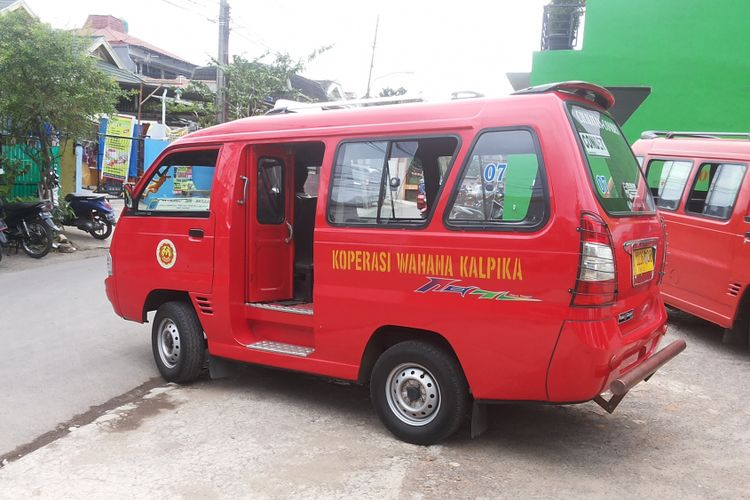
\includegraphics[scale=0.3]{angkot}
	\caption[Angkot yang sedang beroperasi]{Angkutan kota (angkot) yang sedang beroperasi}
	\label{fig:angkot}
\end{figure}

Walaupun begitu, ada salah satu kelemahan fatal dari sistem ini, yaitu kurangnya akses informasi yang dapat dilihat terlebih dahulu oleh penumpang angkot sebelum menggunakan layanan tersebut. Sistem angkot yang ada bergantung pada kode angka yang ada di angkot tersebut (biasanya ditempelkan pada kaca jendela angkot.) Masing-masing kode angka yang berbeda menandakan bahwa angkot tersebut akan menempuh rute yang berbeda. Hal ini menjadi sebuah kekurangan karena sampai sekarang pun tidak ada akses informasi yang konsisten untuk rute mana saja yang ditempuh angkot-angkot dengan kode angka tertentu---informasi yang ada saat ini hanyalah tulisan lokasi rute yang ditempuh oleh angkot, yang tidak hanya mengandalkan penumpang angkot untuk hafal letak-letak dari lokasi tersebut, tetapi juga terkadang bahkan tidak ada sama sekali, seperti pada Gambar \ref{fig:angkot}, di mana angkot yang ditunjukkan pada gambar tersebut tidak memiliki teks lokasi rute baik di kaca depan, samping, maupun belakang dari angkot tersebut.

\begin{figure}[h]
	\centering
	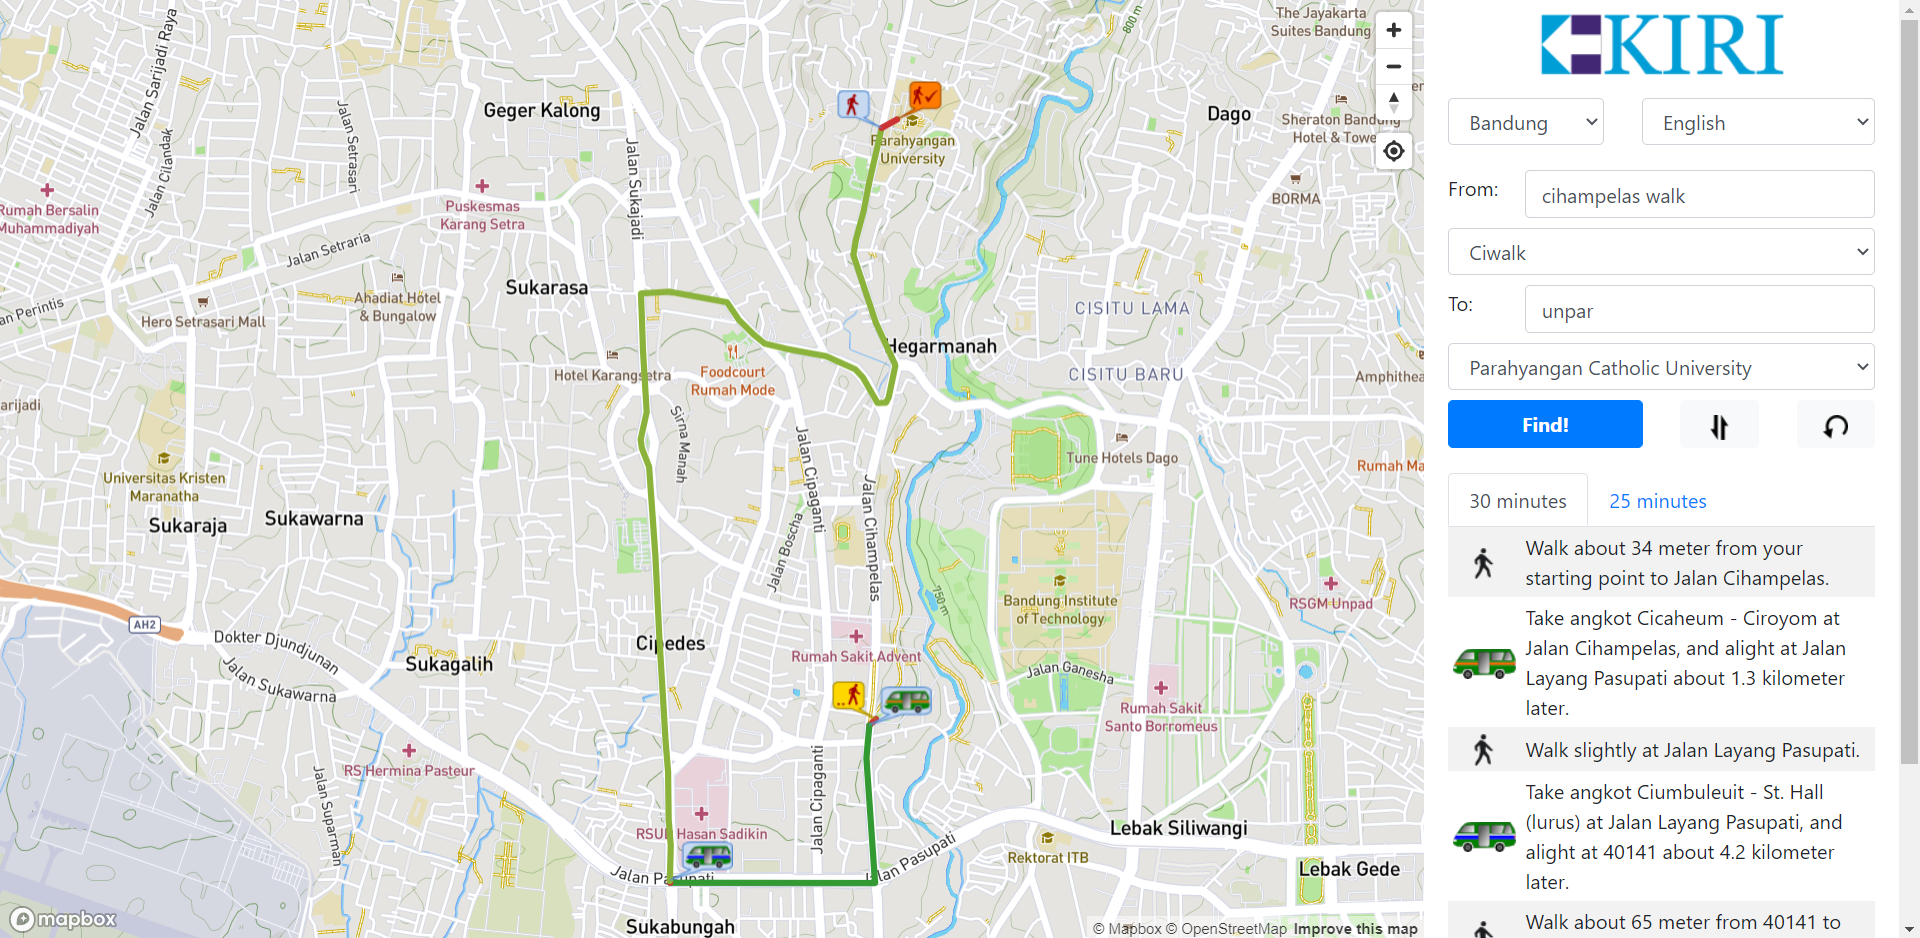
\includegraphics[width=\textwidth]{projectkiri}
	\caption[Tampilan halaman web KIRI]{Tampilan halaman web \href{https://projectkiri.id}{KIRI}, menunjukkan rute dari Cihampelas Walk ke Universitas Katolik Parahyangan.}
	\label{fig:kiripage}
\end{figure}

Permasalahan inilah yang merupakan tujuan dari pencetusan Project KIRI. Project KIRI (atau KIRI saja) adalah sebuah perkakas berbasis web yang dapat menunjukkan rute angkot dari satu titik ke titik lain, mulai dari seberapa jauh pengguna harus berjalan untuk menaiki angkot yang bersangkutan, di mana pengguna harus naik atau turun, seberapa jauh lagi pengguna harus berjalan sampai ke titik tujuan, dan seberapa lama estimasi waktu perjalanan yang akan ditempuh.

Pada skripsi ini akan dibuat sebuah perkakas \textit{command line} (\textit{command line tool}) yang dapat menjalankan fungsi-fungsi API dari Project KIRI Keseluruhan dari perangkat lunak ini akan dibangun dalam bahasa C.

\section{Rumusan Masalah}
\begin{itemize}
	\item Sejauh mana KIRI dapat membantu penumpang angkot untuk mengetahui rute angkot?
	\item Bagaimana membangun perkakas \textit{command line} yang dapat mengimplementasikan fitur-fitur API KIRI dalam bahasa C?
\end{itemize}

\section{Tujuan}
\begin{itemize}
	\item Mengetahui sejauh mana KIRI dapat membantu penumpang angkot untuk mengetahui rute angkot dengan lebih baik.
	\item Membangun perkakas \textit{command line} yang dapat mengimplementasikan fitur-fitur API KIRI dalam bahasa C.
\end{itemize}

\section{Deskripsi Perangkat Lunak}
Tuliskan deksripsi dari perangkat lunak yang akan anda hasilkan. Apa saja fitur yang disediakan oleh PL tersebut dan apa saja kemampuan dari PL tersebut. Perhatikan contoh di bawah ini:

Perangkat lunak akhir yang akan dibuat memiliki fitur minimal sebagai berikut:
\begin{itemize}
	\item Pengguna dapat melihat denah Musem Geologi Bandung dalam bidang dua dimensi. Sedangkan pengunjung direpresentasikan menggunakan lingkaran-lingkaran kecil (tidak menggunakan gambar manusia yang diambil dari atas)
	\item Pengguna dapat memunculkan atau menghilangkan gambar {\it flow tiles} pada denah museum. 
	\item Pengguna dapat mengatur jalannya simulasi: memulai(start) simulasi, menunda(pause) simulasi, melanjutkan(continue) simulasi, maupun menghentikan(stop) simulasi
	\item Pengguna dapat mengatur banyaknya pengunjung di dalam museum, baik melalui perubahan frekuensi kedatangan pengunjung maupun menambahkan dan menghapus pengunjung satu-persatu secara manual.
	\item Posisi kamera dapat diubah (pergerakan di bidang tiga dimensi) sehingga pengguna dapat melihat simulasi di museum dari berbagai arah. 
	\item Posisi kamera dapat diubah untuk emngikuti perjalanan seorang pengunjung di dalam 
	\item Pengguna dapat memilih apakah akan menggunakan teknik {\it flow tiles} atau tidak pada saat simulasi berlangsung
	\item Jenis {\it flow tiles} yang digunakan dapat diubah-ubah pada saat simulasi sedang berlangsung
		
\end{itemize}

\section{Detail Pengerjaan Skripsi}
Tuliskan bagian-bagian pengerjaan skripsi secara detail. Bagian pekerjaan tersebut mencakup awal hingga akhir skripsi, termasuk di dalamnya pengerjaan dokumentasi skripsi, pengujian, survei, dll.

Bagian-bagian pekerjaan skripsi ini adalah sebagai berikut :
	\begin{enumerate}
		\item Melakukan survei ke Museum Geologi Bandung untuk mendapatkan denah serta mengetahui perilaku pengunjung museum secara umum (arah perjalanan, kecepatan, lama melihat objek, dll)
		\item Melakukan analisis pada hasil survei terhadap pergerakan pengunjung di museum dan membuat rancangan denah di komputer yang dilengkapi dengan penghalang dan objek di museum.
		\item Melakukan studi literatur mengenai sifat kolektif suatu kerumunan, teknik {\it social force model} dan teknik {\it flow tiles}
		\item Mempelajari bahasa pemrograman C++ dan cara menggunakan framework OpenSteer
		\item Merancang pergerakan kerumunan di dalam museum menggunakan teknik {\it social force model} dan {\it flow tiles} serta menggunakan teknik lainnya seperti konsep pathway dan waypoints. Selain itu, dirancang pula adanya waktu tunggu (pada saat pengunjung melihat objek di museum) dan cara pembuatan jalur bagi setiap individu pengunjung
		\item Melakukan analisa dan merancang struktur data yang cocok untuk menyimpan penghalang (obstacle)
		\item Mengimplementasikan keseluruhan algoritma dan struktur data yang dirancang, dengan menggunakan framework OpenSteer 
		\item Melakukan pengujian (dan eksperimen) yang melibatkan responde untuk menilai hasil simulasi secara kualitatif
		\item Menulis dokumen skripsi
	\end{enumerate}

\section{Rencana Kerja}
Rincian capaian yang direncanakan di Skripsi 1 adalah sebagai berikut:
\begin{enumerate}
\item
\item
\item
\end{enumerate}

Sedangkan yang akan diselesaikan di Skripsi 2 adalah sebagai berikut:
\begin{enumerate}
\item
\item
\item
\end{enumerate}

\vspace{1cm}
\centering Bandung, \tanggal\\
\vspace{2cm} \nama \\ 
\vspace{1cm}

Menyetujui, \\
\ifdefstring{\jumpemb}{2}{
\vspace{1.5cm}
\begin{centering} Menyetujui,\\ \end{centering} \vspace{0.75cm}
\begin{minipage}[b]{0.45\linewidth}
% \centering Bandung, \makebox[0.5cm]{\hrulefill}/\makebox[0.5cm]{\hrulefill}/2013 \\
\vspace{2cm} Nama: \makebox[3cm]{\hrulefill}\\ Pembimbing Utama
\end{minipage} \hspace{0.5cm}
\begin{minipage}[b]{0.45\linewidth}
% \centering Bandung, \makebox[0.5cm]{\hrulefill}/\makebox[0.5cm]{\hrulefill}/2013\\
\vspace{2cm} Nama: \makebox[3cm]{\hrulefill}\\ Pembimbing Pendamping
\end{minipage}
\vspace{0.5cm}
}{
% \centering Bandung, \makebox[0.5cm]{\hrulefill}/\makebox[0.5cm]{\hrulefill}/2013\\
\vspace{2cm} Nama: \makebox[3cm]{\hrulefill}\\ Pembimbing Tunggal
}
\end{document}

